
% This LaTeX was auto-generated from MATLAB code.
% To make changes, update the MATLAB code and republish this document.

\documentclass{article}
\usepackage{graphicx}
\usepackage{color}

\sloppy
\definecolor{lightgray}{gray}{0.5}
\setlength{\parindent}{0pt}

\begin{document}

    
    \begin{verbatim}
clear all;clc

k = 5;
b = 2;
m = 1;

A = [0 1; -k/m -b/m];
B = [0; 1/m];
C = [1 0];

% initialization
t = 0:0.01:10; % time step 0.01
nt = length(t);
dt = t(2) - t(1);
x(:,1) = [0.2 1.0];
y(:,1) = C*x(:,1);

Mp = 2; % percent overshoot
Ts = 2; % transient time
Mlog = log(Mp/100);
MlogSquared = Mlog^2;
zeta = sqrt(MlogSquared/(pi^2+MlogSquared));
w0 = 4/(Ts*zeta);
P = roots([1 2*zeta*w0 w0^2])
K = place(A,B,P)
A1 = A - B*K;
eig(A1)

yss = 1; % steady state response
kg = -yss/(C*inv(A-B*K)*B);

for i = 1:nt-1
r(i) = 1;
u(i) = -K*x(:,i) + kg*r(i);
x_dot(:,i) = A*x(:,i) + B*u(i);
x(:,i+1) = x(:,i) + x_dot(:,i)*dt;
y(:,i+1) = C*x(:,i+1);
end

figure
plot(t,y,'b','linewidth',2)
set(gca,'fontsize',18)
legend({'$x$'},'Interpreter', 'latex')
title('state-feedback')
legend boxoff
xlabel('Time (s)')
% print(gcf,'state_feedback.png','-dpng','-r300');
\end{verbatim}

        \color{lightgray} \begin{verbatim}
P =

  -2.0000 + 1.6061i
  -2.0000 - 1.6061i


K =

    1.5796    2.0000


ans =

  -2.0000 + 1.6061i
  -2.0000 - 1.6061i

\end{verbatim} \color{black}
    
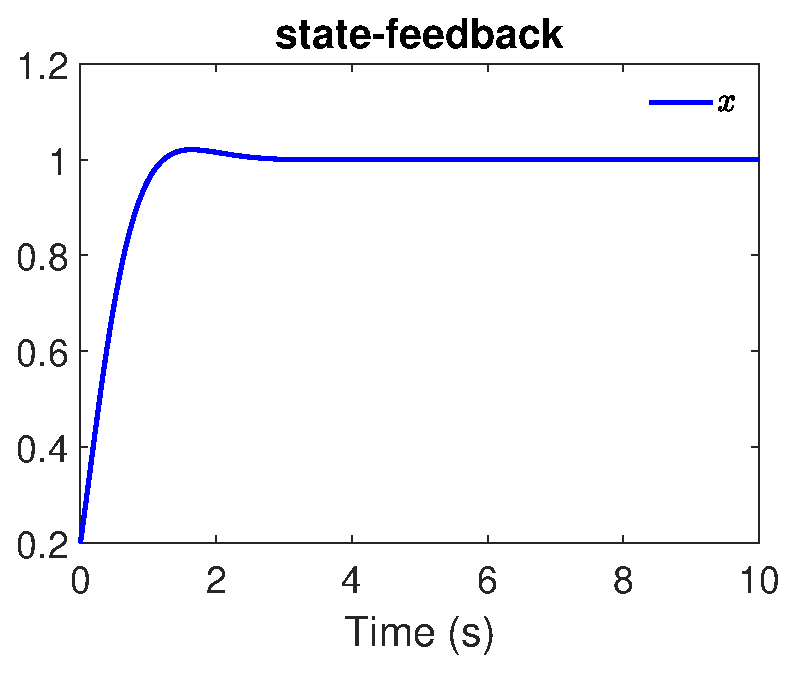
\includegraphics [width=4in]{mbk_state_feedback_01.eps}



\end{document}

